

%Quellen:
% https://tex.stackexchange.com/questions/5339/how-to-specify-font-size-less-than-10pt-or-more-than-12pt
% https://guides.github.com/introduction/flow/
% https://www.computerhope.com/issues/ch001927.htm
% https://git-scm.com/doc --> Website von Git, Programm Download, Buch, Doki etc.


% extarticle -> kleiner Schriftgrösse
\documentclass[a4paper, 8pt]{extarticle}

%Packages sind in separaten .sty Dateine abgespeichert
\usepackage{include/Vorlage_Cheatsheet}
\usepackage{include/report}
\usepackage{fancybox}

%\setlist{leftmargin=3mm, nosep}

\title{ZF AEMBS}
\author{Riccardo Degiacomi}

\begin{document}
    % Formatierung 3 Spalten
    \begin{multicols*}{3}
        \section{Git auf Windows Installieren}
            %Quelle: 
                \begin{enumerate}
                    \item   Öffne https://git-scm.com
                        \begin{itemize}
                            \item   (Website stellt Buch zu Git zur Verfügung, Dokumentation etc.)
                            \item   (repository von Git auf Github\\
                            https://github.com/git/git)
                        \end{itemize}
                    \item   Lade das Programm herunter
                    \item   Installiere das Programm Notepad++
                    \item   Starte die Installation
                    \item   "Adjusting your PATH environment"\\Wähle: "Git from command line and also from 3rd-party software"\\ermöglicht das benutzen von Git mit Git Bash und cmd
                    \item   Bei Choosing HTTPS transport backend standard lassen, also:\\Use the OpenSSL library ausgewählt lassen.
                    \item   Bei Configuring the line ending conversions wähle:\\Checkout Windows-style, commit Unix-style line endings
                    \item   Configuring the terminal emulator to use with Git Bash wähle:\\Use MinTTY (the default terminal of MSYS2).
                    \item   Bei Configuring extra options\\ so lassen wie es ist.
                \end{enumerate}
asdfasdfasdf
        \section{Git Konfigurieren und mit einem Repository verbinden}
                \begin{enumerate}
                    \item   Windows CMD (Kommandozeilenprogramm) verwenden um zu Ordner navigieren, 
                            den man hochladen möchte.\\
                            Mit dir kann man den Pfad und alle Inhalte des Ordners anzeigen lassen. 
                                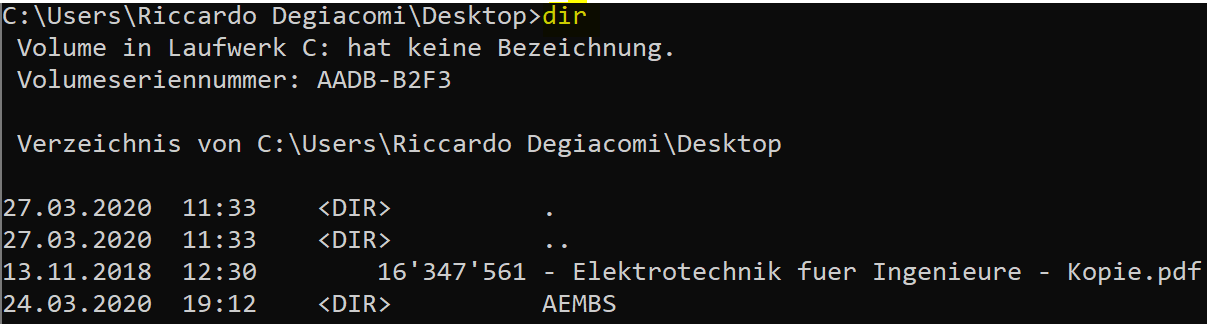
\includegraphics[width=1\linewidth, left]{img/cmd_befehle_dir}
                            mit \Ovalbox{cd} verzeichnisname kann man in ein anderes Verzeichnis oder einen Ordner wechseln. 
                                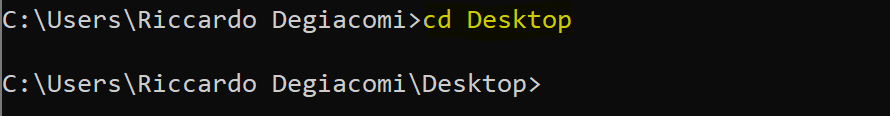
\includegraphics[width=1\linewidth, left]{img/cmd_befehle_cd}
                    \item   Git Benutzernamen Konfigurieren:\\
                            \Ovalbox{git config --global user.name username} \\
                                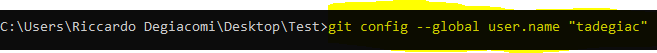
\includegraphics[width=1\linewidth, left]{img/git_config_username.PNG}
                    \item   E-Mail angeben:\\
                            git config --global user.email "<your e-mail>"
                            Jetzt ist es einem möglich sich mit einem Git Repository zu verbinden.
                                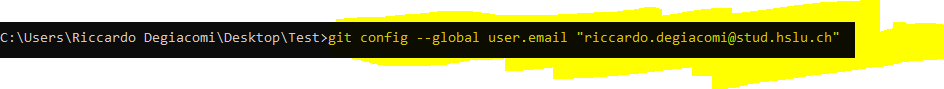
\includegraphics[width=1\linewidth, left]{img/git_config_email.PNG}
                    \item   Gewünschtes Git-Repository öffnen und kopieren (Ctrl+C)
                                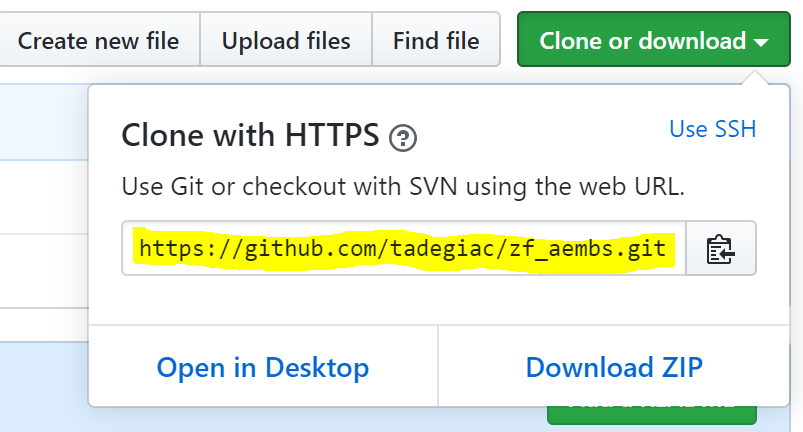
\includegraphics[width=1\linewidth, left]{img/git_repository_via_https.PNG}
                    \item   Zurück in der Kommandozeile\\ (im richtigen Verzeichnis $\rightarrow$ Ordner für Projekt)
                            mit dem Befehl:\\ git clone\\
                            Adresse des repositories einfügen.
                                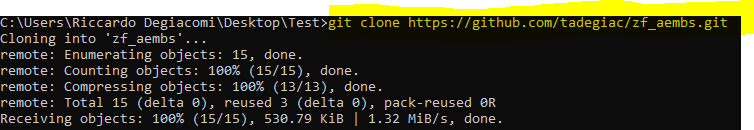
\includegraphics[width=1\linewidth, left]{img/git_config_clone.PNG}
                            Nach dem Ausführen dieses Schrittes hat man jetzt einen neuen Ordner im Verzeichnis
                            mit dem Namen des Git repositories.
                    \item   Als nächstes sollte man in das Verzeichnis dieses Ordners wechseln (wieder mit cd).
                            Im Verzeichnis kann man nun den befehl:\\
                            git remote in der Kommandozeile eingeben. \\
                                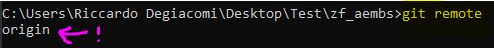
\includegraphics[width=1\linewidth, left]{img/git_remot.PNG}
                            Wenn alle bisherigen Schritte korrekt ausgeführt wurden, sollte jetzt
                            origin in der Kommandozeile stehen.
                            Mit git remot -v kann man die aliase anzeigen lassen.
                                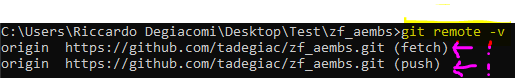
\includegraphics[width=1\linewidth, left]{img/git_remote_-V.PNG}
                            Jetzt ist man mit dem Repository verbunden und kann Dateine pullen und pushen.
                \end{enumerate}
            
            \section{Eine neue Datei erstellen und in das repository auf Github pushen}
                 \begin{enumerate}  
                    \item   Um ein neues file zu erstellen kann man z.B:\\
                            start notepad++ example.txt\\
                            eingeben.\\
                                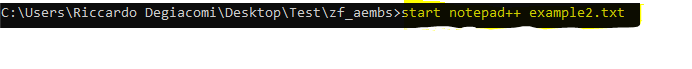
\includegraphics[width=1\linewidth, left]{img/cmd_start_programm.PNG} 
                    \item   Schreibe etwas in den Texteditor und speichere die Datei
                    \item   Tippe folgenden Befehl in die Konsole ein:\\
                            git status\\
                                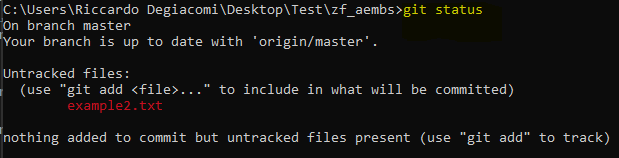
\includegraphics[width=1\linewidth, left]{img/git_status.PNG} 
                    \item   Um dem Programm mitzuteilen, dass wir diese Datei in das Repository comitten/laden möchten 
                            kann man diesen Befehl eingeben:\\
                            git add example.txt\\
                            (statt den namen der datei kann man auch einen ganzen ordner hochladen ;)\\
                                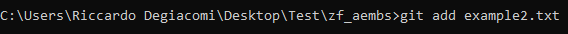
\includegraphics[width=1\linewidth, left]{img/git_add.PNG} 
                    \item   Nachtem enter gedrückt wurde weiss das Programm dass diese Datei neu ist und hochgeladen werden soll.
                            Dieser Vorgang wird auch als staging bezeichnet.
                            Wichtig ist, es ist noch ein anderer Befehl nötig um diese dann wirklich hochzuladen.
                            Dies kann man sehen wenn man erneut git status eingibt. \\
                                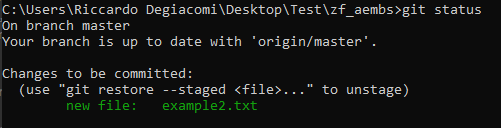
\includegraphics[width=1\linewidth, left]{img/git_status_2.PNG}                          
                    \item   Um die Datei nun hoch zu laden verwendet man diesen Befehl:\\
                            git commit -m "blabla"\\
                            das -m ist dazu da dass nicht irgend ein komischer editor geöffnet wird den scheinbar niemand versteht.
                            Das Zeugs in den Gänsefüsschen ist eine Art Kommentar den man zur Datei schreiben kann.
                                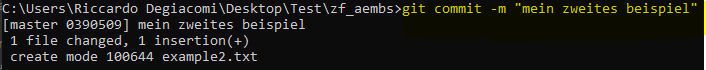
\includegraphics[width=1\linewidth, left]{img/git_commit.PNG}
                    \item   Nach dem Commit kann man mit folgendem Befehl die Datei ins repository laden:\\
                            git push\\
                                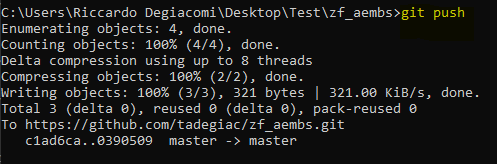
\includegraphics[width=1\linewidth, left]{img/git_push.PNG}\\
                            Wenn der push funktioniert hat sieht das ganz in etwa so aus:
                                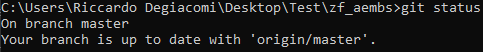
\includegraphics[width=1\linewidth, left]{img/git_status_3.PNG}\\
                                Die Änderungen im repository sehen so aus:
                                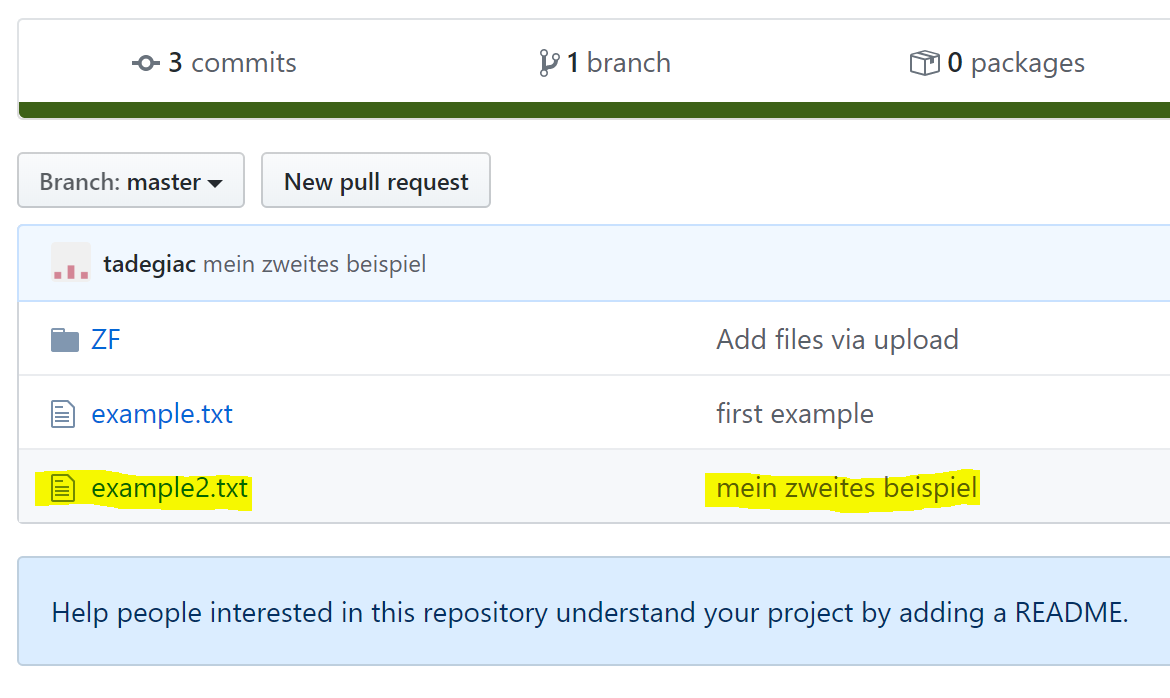
\includegraphics[width=1\linewidth, left]{img/wennallesobeisch.PNG}:
                 \end{enumerate}

            \section{Einen Branch erstellen}    
                 \begin{enumerate}
                    \item   Im Git master Verzeichnis folgendes eingeben:\\
                            git branch branchname\\
                                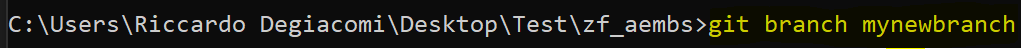
\includegraphics[width=1\linewidth, left]{img/git_branch_mynewbranch.PNG}\\
                            Dies erstellt einen branch. Dieser ist allerdings momentan nur lokal abgespeichert.
                    \item   Als nächstes muss man noch in den neu erstellten Branch wechseln. Dies kann mit folgendem Befehl
                            bewerkstelligt werden:\\
                            git checkout branchname\\
                                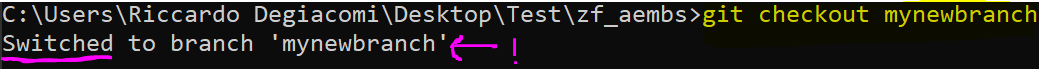
\includegraphics[width=1\linewidth, left]{img/git_checkout_branchname.PNG}\\
                            Wenn man möchte kann man beispielsweise die .txt Datei von Kap.3 ein wenig erweitern 
                            und abspeichern. Wenn alles funktioniert hat ist im Master nichts von der Änderung zu sehen, 
                            und der Branch ist auch nicht im Repository auffindbar. \\ 
                    \item   Überprüfen ob branch bereits auf Repository:\\
                            git branch -a\\
                                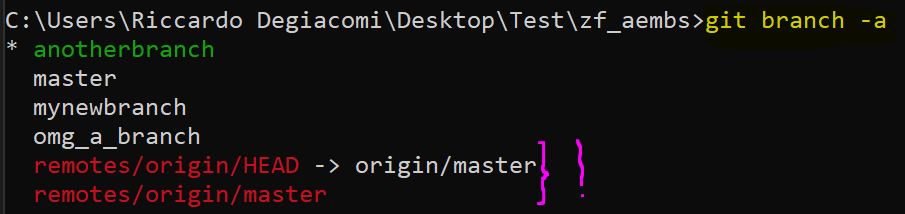
\includegraphics[width=1\linewidth, left]{img/git_branch_branch-a.PNG}\\
                            Man kann zur Sicherheit auch im Repository nachschauen.\\
                                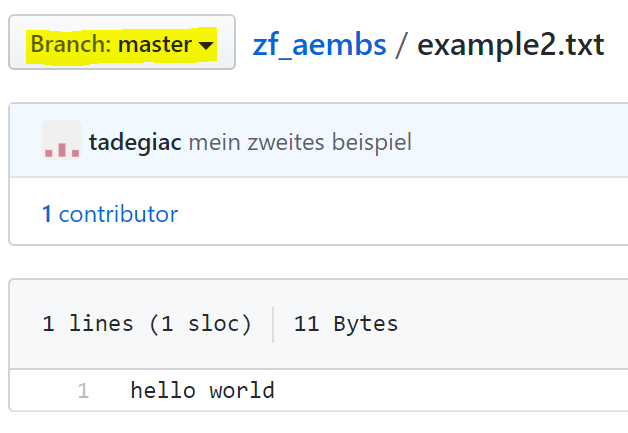
\includegraphics[width=1\linewidth, left]{img/git_branch_example2_master.PNG}\\   
                    \item   Branch auf repository pushen:\\
                            git push --set-upsteram origin branchname\\
                                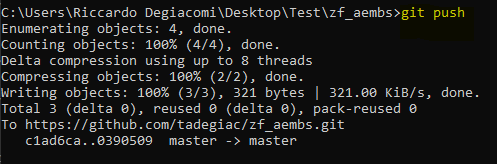
\includegraphics[width=1\linewidth, left]{img/git_push.PNG}\\
                            Nach dem pushen kann man überprüfen ob der erstellte branch auch wirklich im repository ist:
                                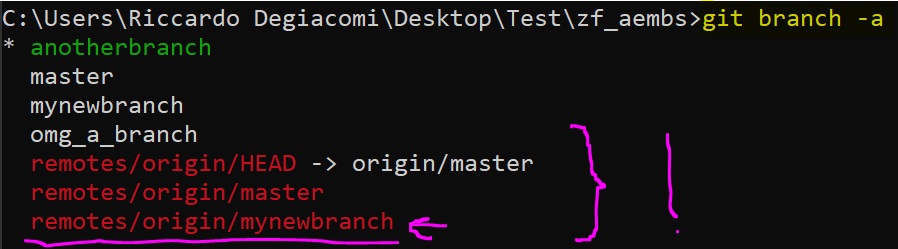
\includegraphics[width=1\linewidth, left]{img/git_push_branch-a_2.PNG}\\
                                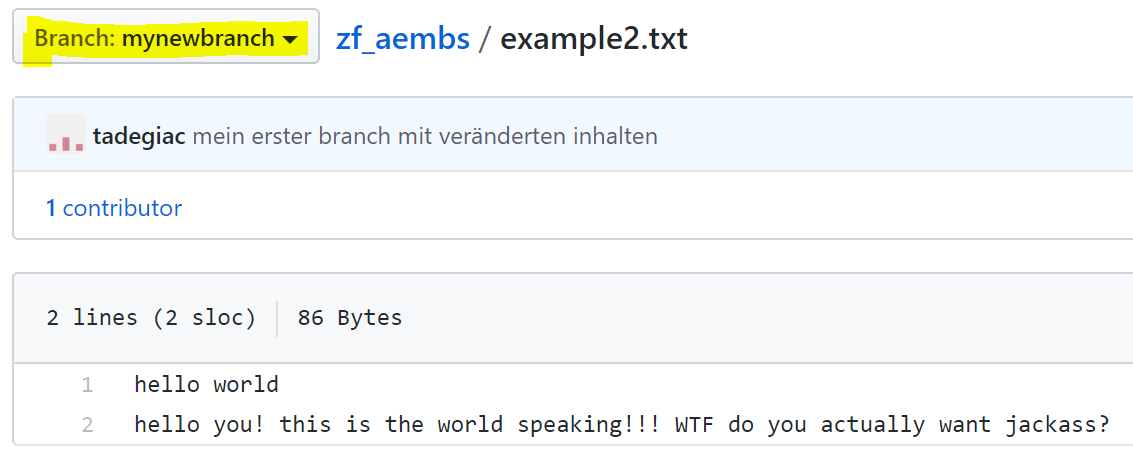
\includegraphics[width=1\linewidth, left]{img/git_branch_example2_mynewbranch.PNG}\\   
                    \item   Zurück zum Master wechseln:\\
                            git checkout Master\\                                   
                 \end{enumerate}

            \section{Branch und Master vereinen}
                 \begin{enumerate}
                    \item  Möchte man die Teile die man im Branch erstellt hat wieder in den Master (oder einen anderen Branch) einfügen,
                            so muss man in das Verzeichnis des Branches wechseln in den die Inhalte eingefügt werden sollen.
                            Dies macht man wieder mit:\\
                            git checkout branchname\\
                                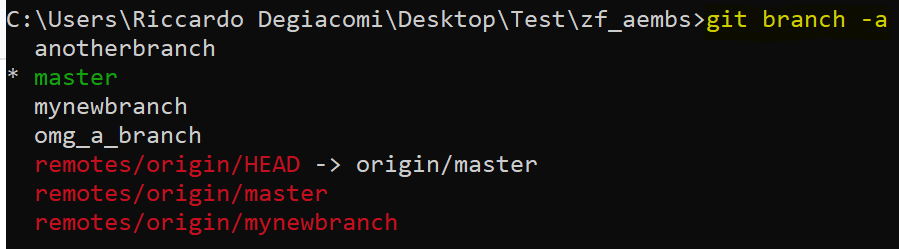
\includegraphics[width=1\linewidth, left]{img/git_merge_destination_branch_check.PNG}\\ 
                    \item   Ist man im Verzeichnis kann man die Dokumente wieder zusammenführen dies nennt man auch merge:\\
                            git merge branchname\\
                                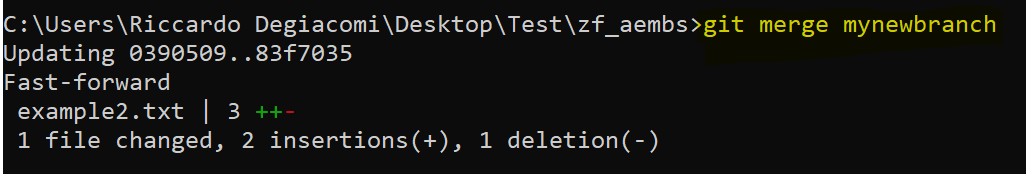
\includegraphics[width=1\linewidth, left]{img/git_merge_merge.PNG}\\ 
                    \item   add\\
                                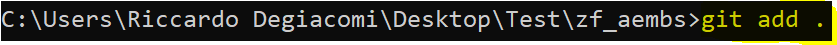
\includegraphics[width=1\linewidth, left]{img/git_merge_add.PNG}\\ 
                    \item   commit\\
                                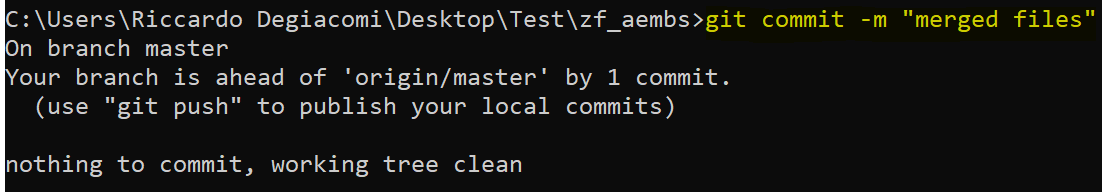
\includegraphics[width=1\linewidth, left]{img/git_merge_commit.PNG}\\ 
                    \item   push\\
                                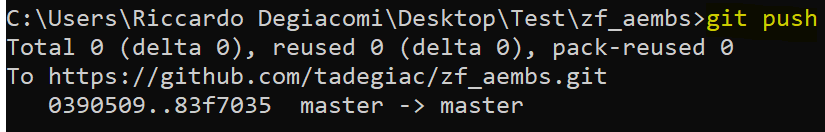
\includegraphics[width=1\linewidth, left]{img/git_merge_push.PNG}\\
                            Auch im repo kann man nun die Änderungen sehen.\\
                                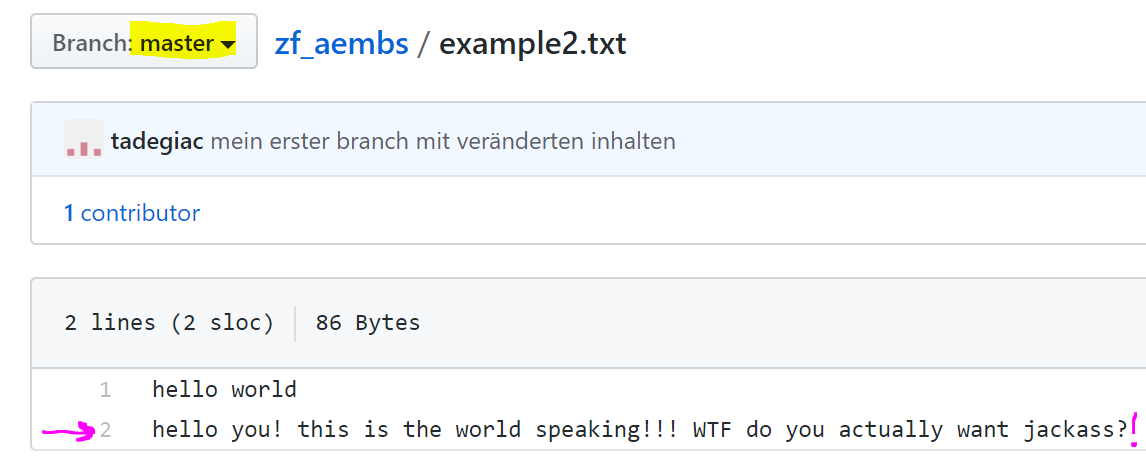
\includegraphics[width=1\linewidth, left]{img/git_merge_master_repo.PNG}\\                
                 \end{enumerate}

            \section{Lokalen Branch \& Branch auf Repo löschen}
                 \begin{enumerate}
                    \item   Lokalen branch löschen (geht nicht solange man sich im Branch den man löschen möchte befindet >.<):\\
                            git branch -d branchname\\
                            Überprüfen in welchem branch man sich befindet.\\
                                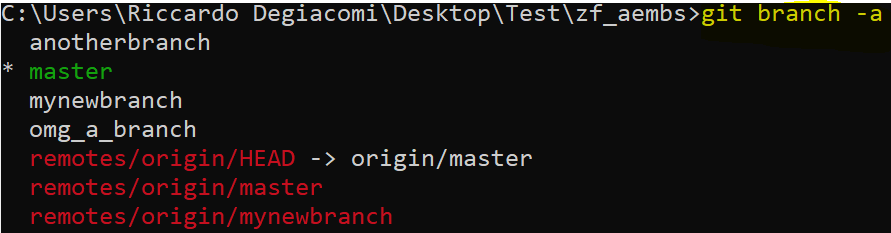
\includegraphics[width=1\linewidth, left]{img/git_delete_branch_local_1.PNG}\\
                            Unbenötigte branches löschen.\\
                                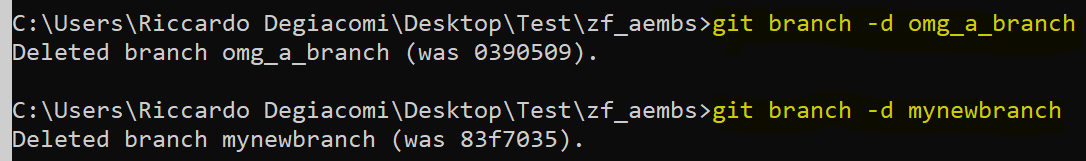
\includegraphics[width=1\linewidth, left]{img/git_delete_branch_local_2.PNG}\\
                            Überprüfen ob branches lokal gelöscht wurden\\
                                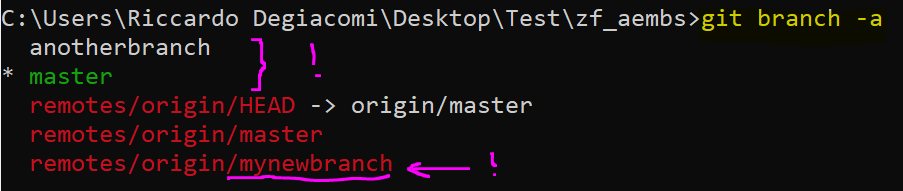
\includegraphics[width=1\linewidth, left]{img/git_delete_branch_local_3.PNG}\\   
                    \item   branch auf Repository löschen:\\
                            git push origin --delete branchname\\
                                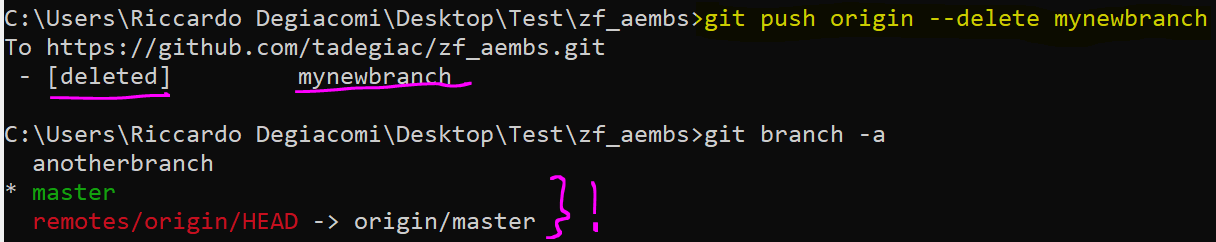
\includegraphics[width=1\linewidth, left]{img/git_delete_branch_remotePNG.PNG}\\ 
                            Überprüfen ob im repo auch weg\\
                                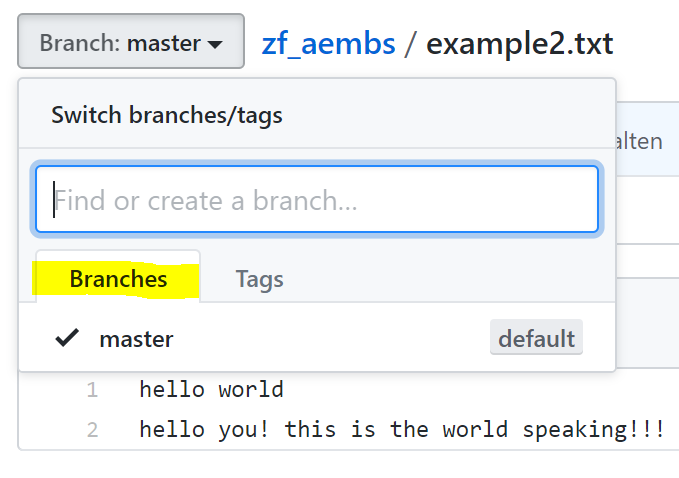
\includegraphics[width=1\linewidth, left]{img/git_delete_branch_remotePNG_repo}\\
                 \end{enumerate}

            \section{Konflikte beim mergen}
                ...todo... 
            \section{Github Workflow}
                 \begin{enumerate}
                    \item   Einen Branch erstellen:\\
                                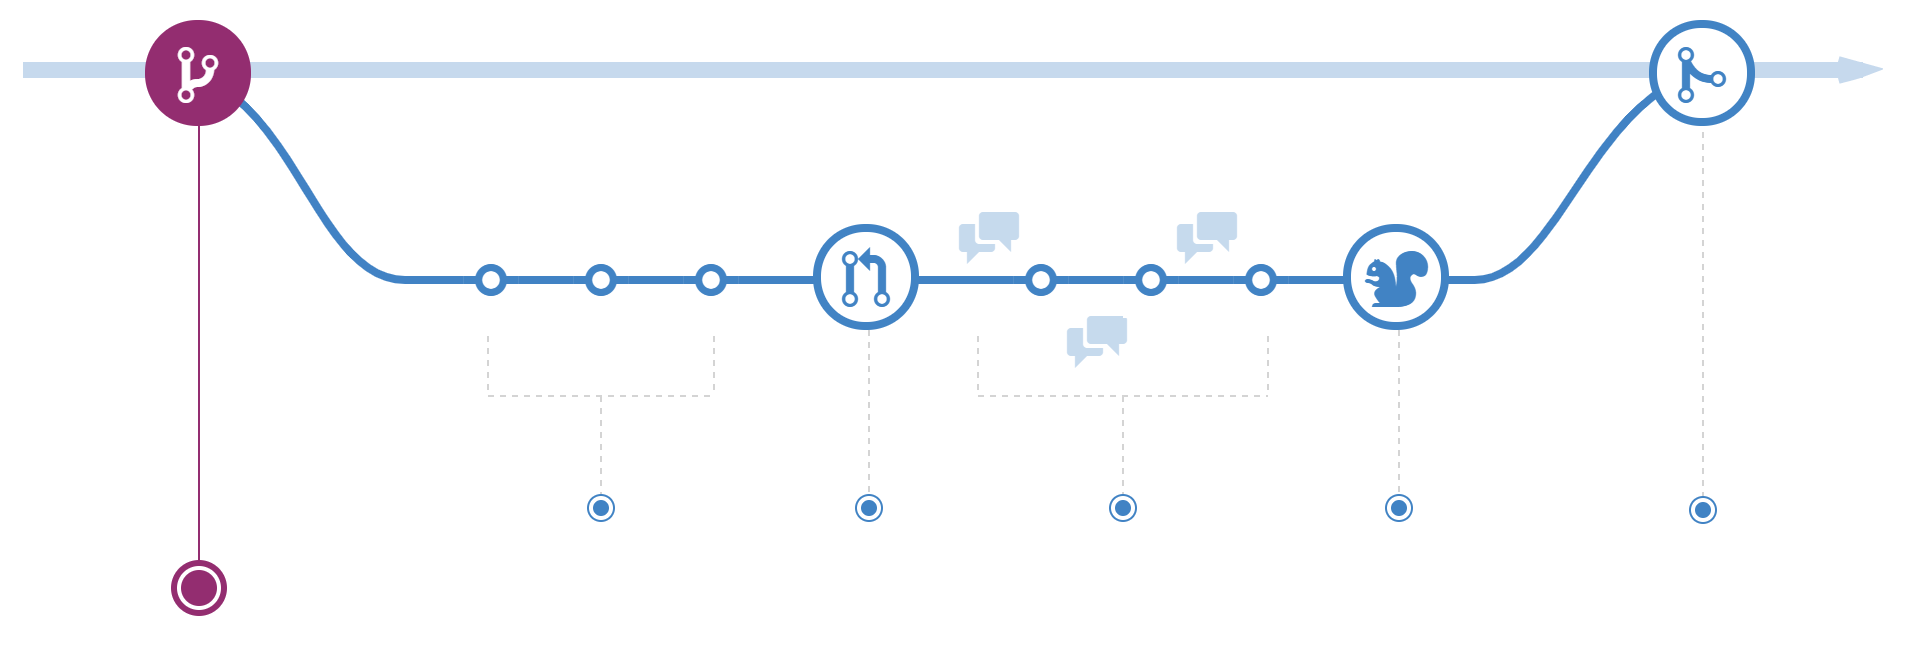
\includegraphics[width=1\linewidth, left]{img/git_workflow_createbranch.PNG}\\
                            Branches erstellt man um neue Idee für ein Projekt ausprobieren zu können,
                            ohne gleich das ganze Projekt verändern zu müssen. Zusätzlich ermöglicht
                            asynchrones zusammenarbeiten an verschiedenen Problemen des selben Projekts.
                            Grundsätzlich sollte man nur vom Master branchen.
                            Der branchname sollte deskriptiv für die Idee sein die im branch verfolg wird damit
                            den anderen Usern klar ist wozu der branch dient. Branchnamen Beispiele: zf-aembs-kapitel-5,
                            aembs-codebeispiele-ledtreiber-interrupts etc.
                    \item   commits hinzufügen:\\
                                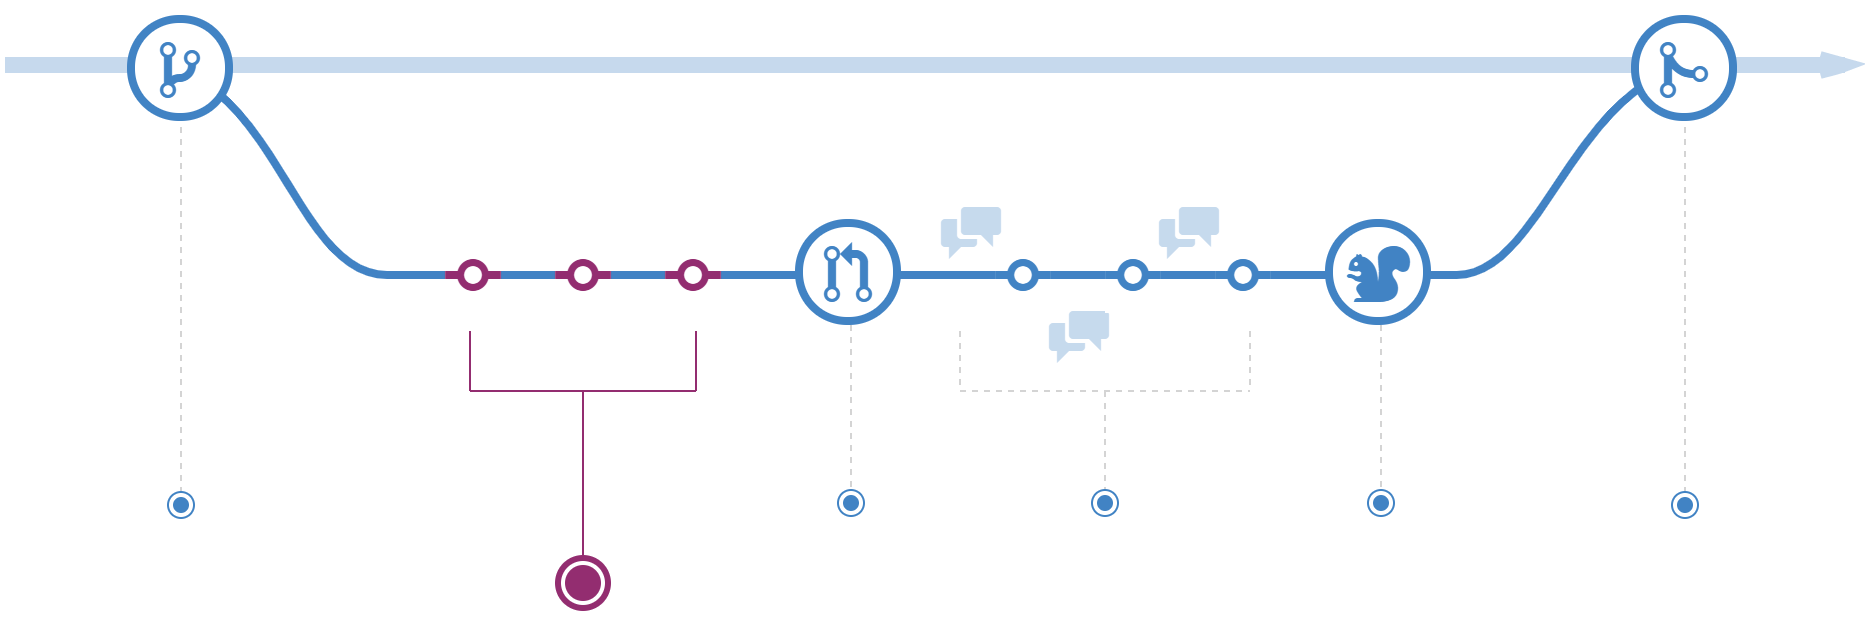
\includegraphics[width=1\linewidth, left]{img/git_workflow_commits}\\
                            Sobald man einen neuen Branch erstellt hat, beginnt man für gewöhnlich an seiner Idee zu arbeiten.
                            Grundsätzlich sollte man nach jeder signifikanten Änderung einen commit machen. Jeder commit wird von
                            git separat aufgeführt. Somit sind die einzelnen Arbeitsschritte als commits aufgeführt. Dies ist äusserst nützlich 
                            da so der Arbeitsfortschritt aufgezeichnet wird. Weiterhin kann man zu jedem commit einen Kommentar schreiben der
                            ebenfalls hinzugefügt wird. So können die einzelnen Teammitglieder nachvollziehen was in welchem Arbeitsschritt 
                            gemacht wurde. Jeder commit wird als separate Änderung gespeichert. Falls Probleme auftreten kann man einzelene
                            commits Rückgängig machen und so "debuggen".
                    \item   pull requests auslösen:\\
                                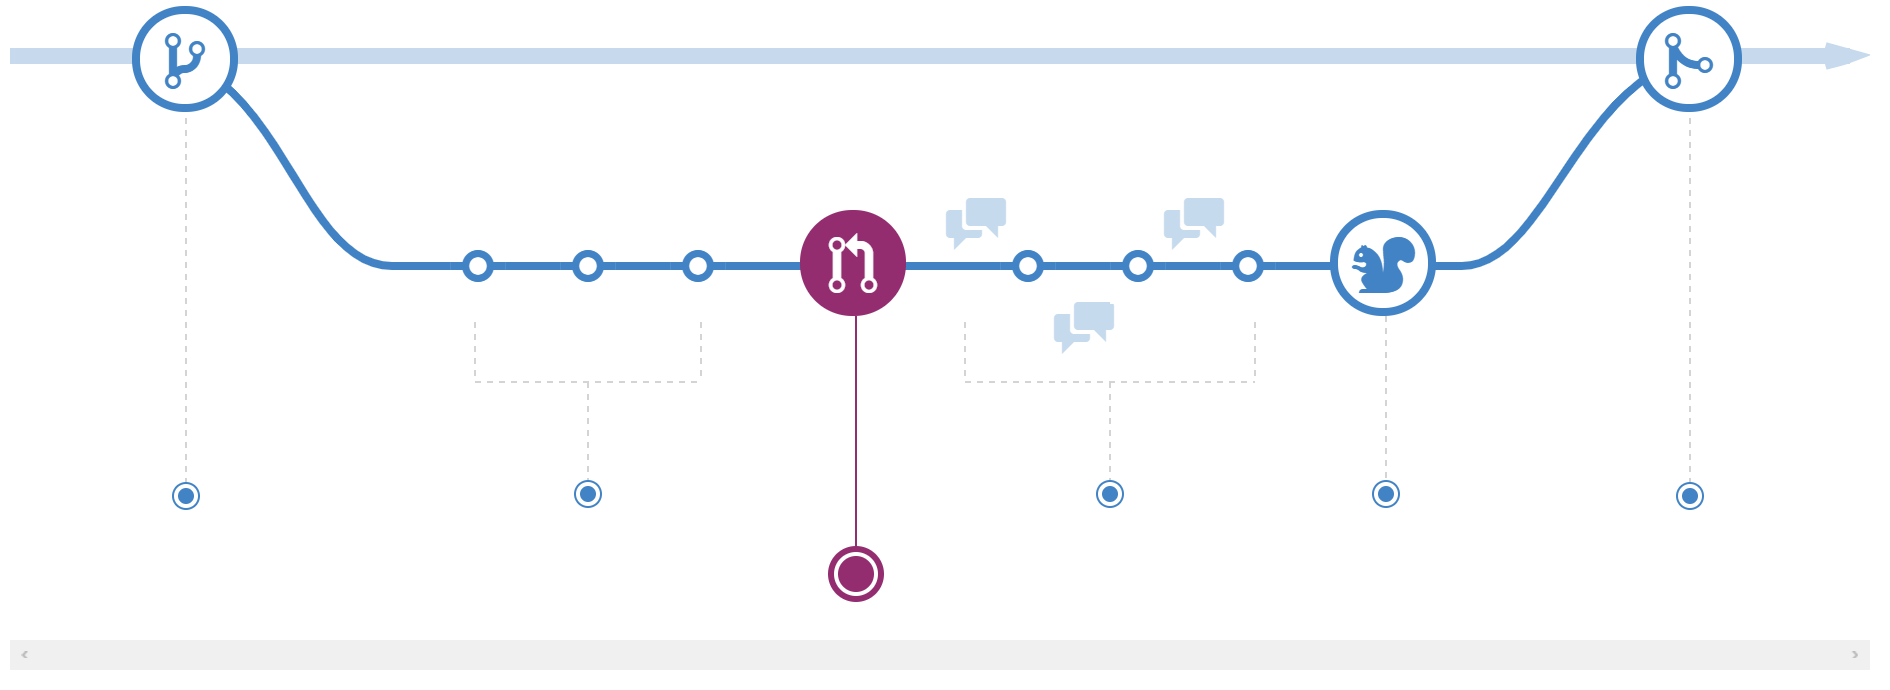
\includegraphics[width=1\linewidth, left]{img/git_workflow_pullrequest.PNG}\\
                            Wenn ein pullrequest akzeptiert wird, wird der master mit dem branch gemerged. Dies bedeutet, dass
                            jeder der am Projekt arbeitet die Änderungen die im master vorgenommen würden sehen kann. Dies dient dazu
                            einen Diskurs auszulösen. Jeder kann die Änderungen betrachte und noch seinen Senf dazugeben.
                            Pullrequests sind nützlich für opensource Projekte mit öffentlichen repositories. Sie helfen ein 
                            codereview zu starten und eine disskusion über vorgeschlagenen Änderungen auszulösen.
                            Es besteht die Möglichkeit pull requests mit bestimmten Schlüsselwörtern (issues) zu verknüpfen.
                            Mehr dazu hier:\\
                            https://help.github.com/en/github/managing-your-work-on-github/linking-a-pull-request-to-an-issue 
                    \item   Den Code disskutieren:
                                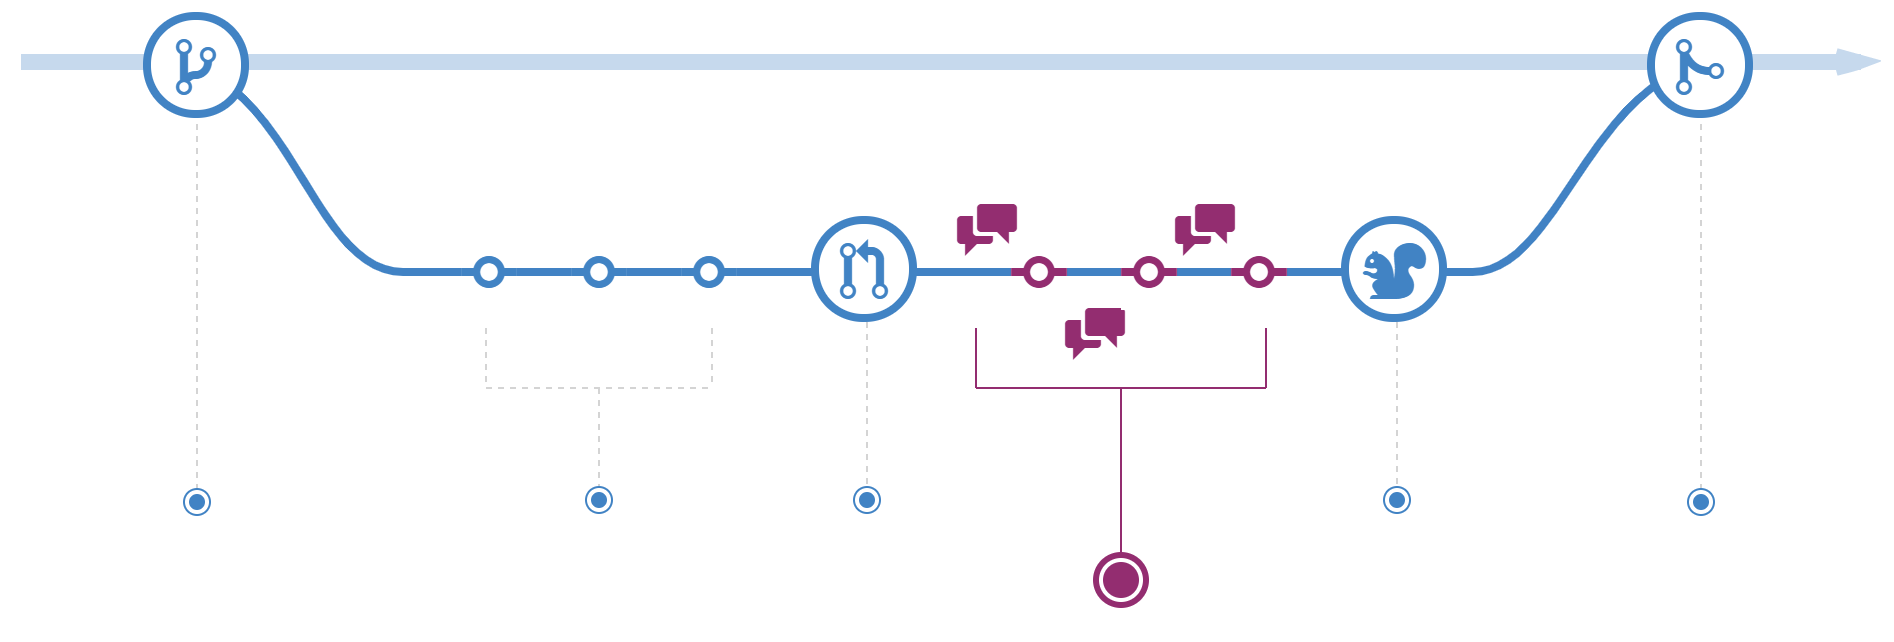
\includegraphics[width=1\linewidth, left]{img/git_workflow_review.PNG}\\
                            Nachdem ein pullrequest ausgelöst wurde und die damit einhergehende Disskusion, kann man 
                            vortlaufend neue commits machen und pullrequests. Das feedback etc. ist ebenfalls ersichtlich 
                            und dient dem Überblick. Pullrequests werdne in Markdown geschrieben (https://de.wikipedia.org/wiki/Markdown)
                    \item   einsetzen (deploy)\\
                                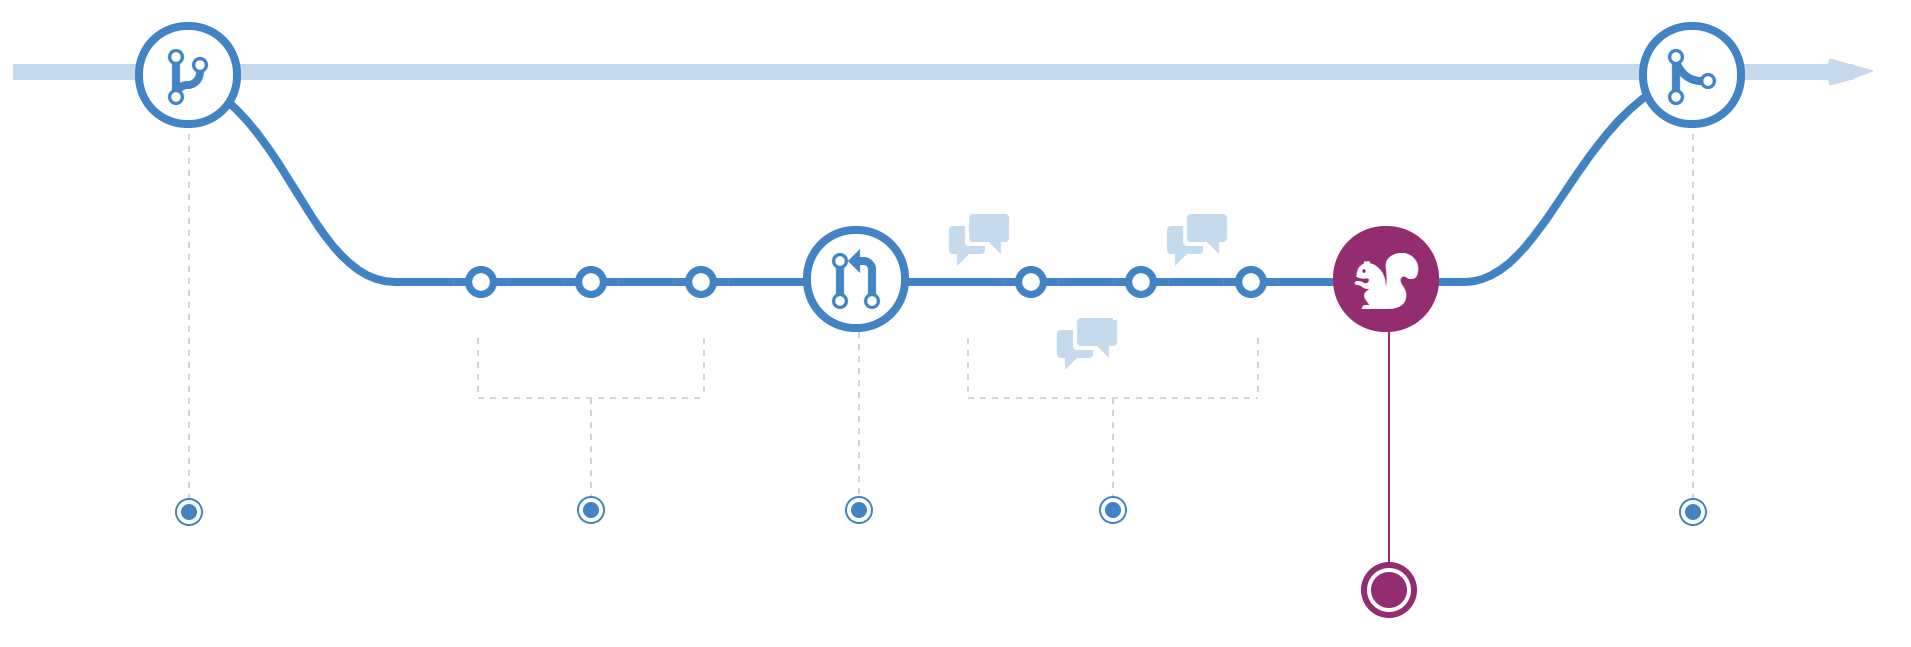
\includegraphics[width=1\linewidth, left]{img/git_workflow_deploy.PNG}\\
                            todo ?
                    \item   merge:\\
                                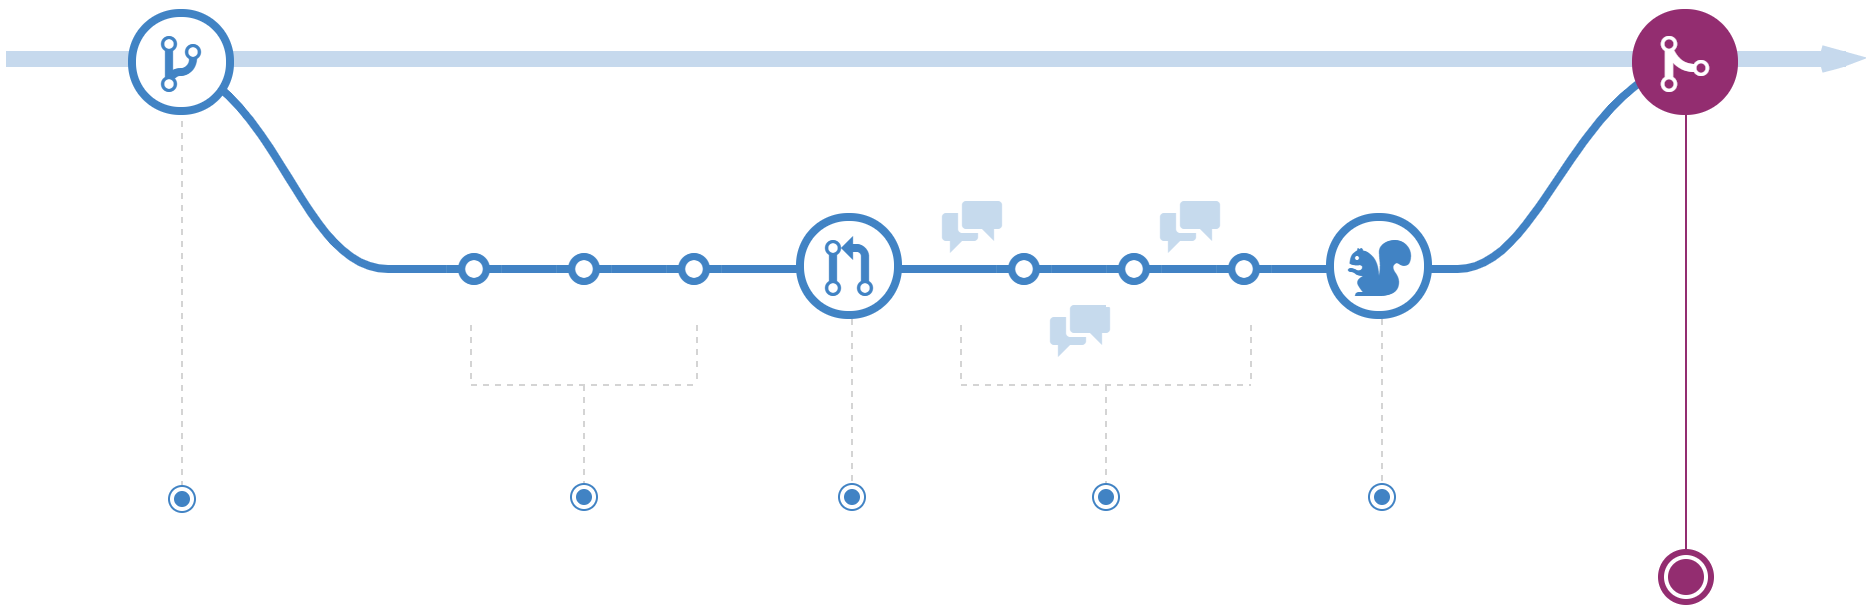
\includegraphics[width=1\linewidth, left]{img/git_workflow_merge.PNG}\\
                            Nachdem die Änderungen akzeptiert wurden kann man diese im Master einbetten.
                            Die pullrequests werden protokolliert, so dass diese nach dem merge noch existieren.
                            Dies ermöglicht das Nachvollziehen und Verstehen der enizelnen Entscheidunen die in der 
                            Vergangenheit getroffen wurden. 

                 \end{enumerate}

    \end{multicols*}
\end{document}